% Options for packages loaded elsewhere
% Options for packages loaded elsewhere
\PassOptionsToPackage{unicode}{hyperref}
\PassOptionsToPackage{hyphens}{url}
%
\documentclass[
  11pt,
  letterpaper,
  DIV=11,
  numbers=noendperiod,
  twoside]{scrartcl}
\usepackage{xcolor}
\usepackage[left=1.1in, right=1in, top=0.8in, bottom=0.8in,
paperheight=9.5in, paperwidth=7in, includemp=TRUE, marginparwidth=0in,
marginparsep=0in]{geometry}
\usepackage{amsmath,amssymb}
\setcounter{secnumdepth}{3}
\usepackage{iftex}
\ifPDFTeX
  \usepackage[T1]{fontenc}
  \usepackage[utf8]{inputenc}
  \usepackage{textcomp} % provide euro and other symbols
\else % if luatex or xetex
  \usepackage{unicode-math} % this also loads fontspec
  \defaultfontfeatures{Scale=MatchLowercase}
  \defaultfontfeatures[\rmfamily]{Ligatures=TeX,Scale=1}
\fi
\usepackage{lmodern}
\ifPDFTeX\else
  % xetex/luatex font selection
  \setmainfont[ItalicFont=EB Garamond Italic,BoldFont=EB Garamond
Bold]{EB Garamond Math}
  \setsansfont[]{EB Garamond}
  \setmathfont[]{Garamond-Math}
\fi
% Use upquote if available, for straight quotes in verbatim environments
\IfFileExists{upquote.sty}{\usepackage{upquote}}{}
\IfFileExists{microtype.sty}{% use microtype if available
  \usepackage[]{microtype}
  \UseMicrotypeSet[protrusion]{basicmath} % disable protrusion for tt fonts
}{}
\usepackage{setspace}
% Make \paragraph and \subparagraph free-standing
\makeatletter
\ifx\paragraph\undefined\else
  \let\oldparagraph\paragraph
  \renewcommand{\paragraph}{
    \@ifstar
      \xxxParagraphStar
      \xxxParagraphNoStar
  }
  \newcommand{\xxxParagraphStar}[1]{\oldparagraph*{#1}\mbox{}}
  \newcommand{\xxxParagraphNoStar}[1]{\oldparagraph{#1}\mbox{}}
\fi
\ifx\subparagraph\undefined\else
  \let\oldsubparagraph\subparagraph
  \renewcommand{\subparagraph}{
    \@ifstar
      \xxxSubParagraphStar
      \xxxSubParagraphNoStar
  }
  \newcommand{\xxxSubParagraphStar}[1]{\oldsubparagraph*{#1}\mbox{}}
  \newcommand{\xxxSubParagraphNoStar}[1]{\oldsubparagraph{#1}\mbox{}}
\fi
\makeatother


\usepackage{longtable,booktabs,array}
\usepackage{calc} % for calculating minipage widths
% Correct order of tables after \paragraph or \subparagraph
\usepackage{etoolbox}
\makeatletter
\patchcmd\longtable{\par}{\if@noskipsec\mbox{}\fi\par}{}{}
\makeatother
% Allow footnotes in longtable head/foot
\IfFileExists{footnotehyper.sty}{\usepackage{footnotehyper}}{\usepackage{footnote}}
\makesavenoteenv{longtable}
\usepackage{graphicx}
\makeatletter
\newsavebox\pandoc@box
\newcommand*\pandocbounded[1]{% scales image to fit in text height/width
  \sbox\pandoc@box{#1}%
  \Gscale@div\@tempa{\textheight}{\dimexpr\ht\pandoc@box+\dp\pandoc@box\relax}%
  \Gscale@div\@tempb{\linewidth}{\wd\pandoc@box}%
  \ifdim\@tempb\p@<\@tempa\p@\let\@tempa\@tempb\fi% select the smaller of both
  \ifdim\@tempa\p@<\p@\scalebox{\@tempa}{\usebox\pandoc@box}%
  \else\usebox{\pandoc@box}%
  \fi%
}
% Set default figure placement to htbp
\def\fps@figure{htbp}
\makeatother


% definitions for citeproc citations
\NewDocumentCommand\citeproctext{}{}
\NewDocumentCommand\citeproc{mm}{%
  \begingroup\def\citeproctext{#2}\cite{#1}\endgroup}
\makeatletter
 % allow citations to break across lines
 \let\@cite@ofmt\@firstofone
 % avoid brackets around text for \cite:
 \def\@biblabel#1{}
 \def\@cite#1#2{{#1\if@tempswa , #2\fi}}
\makeatother
\newlength{\cslhangindent}
\setlength{\cslhangindent}{1.5em}
\newlength{\csllabelwidth}
\setlength{\csllabelwidth}{3em}
\newenvironment{CSLReferences}[2] % #1 hanging-indent, #2 entry-spacing
 {\begin{list}{}{%
  \setlength{\itemindent}{0pt}
  \setlength{\leftmargin}{0pt}
  \setlength{\parsep}{0pt}
  % turn on hanging indent if param 1 is 1
  \ifodd #1
   \setlength{\leftmargin}{\cslhangindent}
   \setlength{\itemindent}{-1\cslhangindent}
  \fi
  % set entry spacing
  \setlength{\itemsep}{#2\baselineskip}}}
 {\end{list}}
\usepackage{calc}
\newcommand{\CSLBlock}[1]{\hfill\break\parbox[t]{\linewidth}{\strut\ignorespaces#1\strut}}
\newcommand{\CSLLeftMargin}[1]{\parbox[t]{\csllabelwidth}{\strut#1\strut}}
\newcommand{\CSLRightInline}[1]{\parbox[t]{\linewidth - \csllabelwidth}{\strut#1\strut}}
\newcommand{\CSLIndent}[1]{\hspace{\cslhangindent}#1}



\setlength{\emergencystretch}{3em} % prevent overfull lines

\providecommand{\tightlist}{%
  \setlength{\itemsep}{0pt}\setlength{\parskip}{0pt}}



 


\setlength\heavyrulewidth{0ex}
\setlength\lightrulewidth{0ex}
\usepackage[automark]{scrlayer-scrpage}
\clearpairofpagestyles
\cehead{
  Brian Weatherson
  }
\cohead{
  Begging the Question and Bayesians
  }
\ohead{\bfseries \pagemark}
\cfoot{}
\makeatletter
\newcommand*\NoIndentAfterEnv[1]{%
  \AfterEndEnvironment{#1}{\par\@afterindentfalse\@afterheading}}
\makeatother
\NoIndentAfterEnv{itemize}
\NoIndentAfterEnv{enumerate}
\NoIndentAfterEnv{description}
\NoIndentAfterEnv{quote}
\NoIndentAfterEnv{equation}
\NoIndentAfterEnv{longtable}
\NoIndentAfterEnv{abstract}
\renewenvironment{abstract}
 {\vspace{-1.25cm}
 \quotation\small\noindent\emph{Abstract}:}
 {\endquotation}
\newfontfamily\tfont{EB Garamond}
\addtokomafont{disposition}{\rmfamily}
\addtokomafont{title}{\normalfont\itshape}
\let\footnoterule\relax
\KOMAoption{captions}{tableheading}
\makeatletter
\@ifpackageloaded{caption}{}{\usepackage{caption}}
\AtBeginDocument{%
\ifdefined\contentsname
  \renewcommand*\contentsname{Table of contents}
\else
  \newcommand\contentsname{Table of contents}
\fi
\ifdefined\listfigurename
  \renewcommand*\listfigurename{List of Figures}
\else
  \newcommand\listfigurename{List of Figures}
\fi
\ifdefined\listtablename
  \renewcommand*\listtablename{List of Tables}
\else
  \newcommand\listtablename{List of Tables}
\fi
\ifdefined\figurename
  \renewcommand*\figurename{Figure}
\else
  \newcommand\figurename{Figure}
\fi
\ifdefined\tablename
  \renewcommand*\tablename{Table}
\else
  \newcommand\tablename{Table}
\fi
}
\@ifpackageloaded{float}{}{\usepackage{float}}
\floatstyle{ruled}
\@ifundefined{c@chapter}{\newfloat{codelisting}{h}{lop}}{\newfloat{codelisting}{h}{lop}[chapter]}
\floatname{codelisting}{Listing}
\newcommand*\listoflistings{\listof{codelisting}{List of Listings}}
\makeatother
\makeatletter
\makeatother
\makeatletter
\@ifpackageloaded{caption}{}{\usepackage{caption}}
\@ifpackageloaded{subcaption}{}{\usepackage{subcaption}}
\makeatother
\usepackage{bookmark}
\IfFileExists{xurl.sty}{\usepackage{xurl}}{} % add URL line breaks if available
\urlstyle{same}
\hypersetup{
  pdftitle={Begging the Question and Bayesians},
  pdfauthor={Brian Weatherson},
  hidelinks,
  pdfcreator={LaTeX via pandoc}}


\title{Begging the Question and Bayesians}
\author{Brian Weatherson}
\date{2001}
\begin{document}
\maketitle
\begin{abstract}
In a recent article Patrick Maher shows that the `depragmatised' form of
Dutch Book arguments for Bayesianism tend to beg the question against
their most interesting anti-Bayesian opponents. I argue that the same
criticism can be levelled at Maher's own argument for Bayesianism.
\end{abstract}


\setstretch{1.1}
The arguments for Bayesianism in the literature fall into three broad
categories. There are Dutch Book arguments, both of the traditional
pragmatic variety and the modern `depragmatised' form. And there are
arguments from the so-called `representation theorems'. The arguments
have many similarities, for example they have a common conclusion, and
they all derive epistemic constraints from considerations about coherent
preferences, but they have enough differences to produce hostilities
between their proponents. In a recent paper, Maher
(\citeproc{ref-Maher1997}{1997}) has argued that the pragmatised Dutch
Book arguments are unsound and the depragmatised Dutch Book arguments
question begging. He urges we instead use the representation theorem
argument as in Maher (\citeproc{ref-Maher1993}{1993}). In this paper I
argue that Maher's own argument is question-begging, though in a more
subtle and interesting way than his Dutch Book wielding opponents.

\section{Bayesianism}\label{bayesianism}

What's a Bayesian? The term these days covers so many different
positions that the only safe course is to strictly define what one means
by the term. The alternative, as the discussion in Walley
(\citeproc{ref-Walley1996}{1996}) shows, is to have one of the least
interesting semantic debates ever held. I define a Bayesian to be one
who is committed to two theses, which I'll call (B1) and (B2).

\begin{description}
\item[(B1)]
Belief comes by degrees.
\item[(B2)]
It is a requirement of consistency that these degrees of belief, or
credences, be consistent with the probability calculus.
\end{description}

I should explain (B2) a little. Historically, Bayesians held that
credences were, or at least ought be, reals in {[}0,~1{]}, and the
function \emph{Bel} which takes any proposition into the agent's
credence in that proposition should be a probability function. Modern
Bayesians, following Levi (\citeproc{ref-Levi1980}{1980}) and Jeffrey
(\citeproc{ref-Jeffrey1983}{1983}), allow that credences can be
imprecise. In this case the consistency requirement is that there be
some precisification of their credences which is a probability function.
(B2) is deliberately ambiguous between the traditional and modern
Bayesian positions, largely because nothing in this debate turns on this
question\footnote{Historically the impetus for allowing imprecise
  credences was the economic distinction between insurable and
  uninsurable risks, as discussed in Knight
  (\citeproc{ref-Knight1921}{1921}), Keynes
  (\citeproc{ref-Keynes1937}{1937}), Tintner
  (\citeproc{ref-Tintner1941}{1941}) and Hart
  (\citeproc{ref-Hart1942}{1942}).}.

There are many other properties that could have been used to define
Bayesians. For example, it could be suggested that it is requirement of
being a Bayesian that one think rules like (B2) are derived by analysing
credences as dispositions to bet. This is suggested by Kaplan
(\citeproc{ref-Kaplan1993}{1993, 320}) to be the ``fundamental Bayesian
insight''. Or it could be argued that being a Bayesian requires some an
extra rule to the effect that credences are updated by
conditionalisation. I haven't included that for two reasons. First, I'm
mostly interested in static constraints on credences, and secondly, some
paradigm Bayesians like Levi (\citeproc{ref-Levi1980}{1980}) and
Fraassen (\citeproc{ref-vanFraassen1989}{1989}) reject this rule in its
fully general form. Finally it might be suggested that Bayesians aren't
those that believe certain principles like (B1) and (B2), but only those
who think these principles provide the foundation for all philosophy of
science. So perhaps my definition is a bit liberal.

Now it is well known that not everyone's a Bayesian. One group of
non-Bayesians who have received too little attention from their Bayesian
rivals are those who accept (B1) but not (B2). That is, theorists who
agree there are such things as credences, and even that credences are
important for philosophy of science, but not that they ought be
constrained by the probability calculus. The most interesting example is
the theory of evidence developed by
(\citeproc{ref-Dempster1967}{Dempster 1967},
\citeproc{ref-Dempster1968}{1968}) and Shafer
(\citeproc{ref-Shafer1976}{1976})

Dempster and Shafer, like many other theorists, think that when we have
no evidence either for or against \emph{p}, we should have low credences
in both \emph{p} and \({\lnot}\)\emph{p}. In the limit case it is
acceptable to have our credence in both \emph{p} and in
\({\lnot}\)\emph{p} set at zero. Now this is in conflict with (B2), for
it is a theorem of the probability calculus that
\emph{Pr}(\emph{p})~+~\emph{Pr}(\({\lnot}\)\emph{p})~=~1, and so by (B2)
it is a requirement of rationality that \emph{Bel}(\emph{p}) +
\emph{Bel}(\({\lnot}\)\emph{p}) = 0.

This intuition about cases where the evidence is low is formalised in a
rather neat theory. For simplicity I'll say how the theory works when we
are interested in finitely many propositions; Shafer shows the infinite
case can be dealt with but it doesn't raise any philosophically
interesting differences. We are interested in \emph{n} propositions, so
the possibility space contains 2\textsuperscript{\emph{n}} `worlds'. A
proposition \emph{A} can be identified in the usual ways with the set of
worlds at which it is true. The Bayesian has us place a normalised
measure on this possibility space, with our credence in \emph{A} being
the measure of the set \emph{A}. In Dempster and Shafer's theory we
place a normalised measure, which they call a `mass function' on the
power set of the worlds, excluding the null set. Our credence in
\emph{A} is calculated as the measure of the set of sets which are
subsets of \emph{A}. So in the simplest case, where we are just
interested in one proposition \emph{p}, the mass function is defined on
\{\{\emph{p}\}, \{\({\lnot}\)\emph{p}\}, \{\emph{p},
\({\lnot}\)\emph{p}\}\}. Complete ignorance is represented by giving
\{\emph{p}, \({\lnot}\)\emph{p}\} mass one, and the other sets mass
zero. Hence both \emph{Bel}(\emph{p}) and
\emph{Bel}(\({\lnot}\)\emph{p}) are zero. On the other hand,
\emph{Bel}(\emph{p}~\({\vee}\)~\({\lnot}\)\emph{p}) will be one, as is
\emph{Bel}(\emph{C}) for any classical tautology \emph{C}. As a
consequence of this we will not have the addition rule.

\begin{description}
\item[\emph{Addition}:]
For disjoint \emph{A}, \emph{B},
\emph{Bel}(\emph{A}~\({\vee}\)~\emph{B})~=~\emph{Bel}(\emph{A})~+~\emph{Bel}(\emph{B})
\end{description}

Since Bayesians believe in \emph{Addition} and some opponents do not,
arguments for Bayesianism should be \emph{inter alia} arguments for
\emph{Addition}. I don't want to argue that Dempster and Shafer's theory
is right. It has some internal problems, particularly with updating,
which make it look not too promising as a general theory of evidence.
The recent collection edited by Yager, Fedrizzi, and Kacprzyk
(\citeproc{ref-Yager1994}{1994}) has papers dealing with many of these
issues for the interested reader. My interest in this theory is merely
to show the kind of theorist the Bayesian must argue against. This is
particularly important when the alleged problem with arguments for
Bayesianism is that they are question-begging.

As a last point about the Dempster-Shafer theory it might be noted that
not only does \emph{Addition} fail for credences, the equivalent rule
for valuing bets also fails. Put formally, let an \emph{A}-bet be a bet
which pays £1 if \emph{A} and nothing otherwise. It is consistent with
the Dempster-Shafer theory to say the value of an \emph{A}-bet is always
£\emph{Bel}(\emph{A}). So on this theory it is not the case that for
disjoint \emph{A}, \emph{B} it is true that the value of an
(\emph{A}~\({\vee}\)~\emph{B})-bet always equals the value of an
\emph{A}-bet plus the value of a \emph{B}-bet.

Since it is sometimes thought there is an argument showing this to be
incoherent, it is worthwhile giving a partial defence of its
consistency. An argument like the following appears, as we'll see, to be
endorsed by Maher. There exists a voucher which is an
(\emph{A}~\({\vee}\)~\emph{B})-bet, a ticket which is an \emph{A}-bet
and a coupon which is a \emph{B}-bet. Now anyone holding the ticket and
the coupon will receive exactly the same payout in all circumstances as
anyone holding the voucher, hence they must have the same value. Hence
the value of the voucher is the value of the ticket plus the value of
the coupon. The problem with this argument is that it assumes the ticket
and the coupon are not what economists call complementary goods. Some
goods, like say compact discs, have more value to a consumer if they
hold certain other goods, like compact disc players. On the
Dempster-Shafer theory, the ticket and the coupon may well be
complementary goods. To anyone holding the ticket, the value of the
coupon is the difference between value of the voucher and the value of
the ticket, that is,
\emph{Bel}(\emph{A}~\({\vee}\)~\emph{B})~-~\emph{Bel}(\emph{A}). This
will in general be greater than its `intrinsic' value
\emph{Bel}(\emph{B}). But this goes no way to showing that its value to
someone without the ticket must be greater than \emph{Bel}(\emph{B}).
This, in rough outline, is the objection Schick
(\citeproc{ref-Schick1986}{1986}) makes to Dutch Book arguments. So
arguments for \emph{Addition} which assume that \emph{A}-bets and
\emph{B}-bets are not complements will beg the question against
proponents of the Dempster-Shafer theory, who have a principled reason
to reject that assumption.

\section{Dutch Book Arguments}\label{dutch-book-arguments}

As I mentioned above, there are three broad categories of arguments for
Bayesianism, two breeds of Dutch Book arguments and `representation
theorem' style arguments. In this section I'll briefly deal with the
Dutch Book arguments before looking at Maher's version of the
representation theorem argument in section 3.

The classic, pragmatic, Dutch Book argument, assumes that appropriate
circumstances exist whereby the amount an agent would be prepared to pay
for any \emph{A}-bet is £\emph{Bel}(\emph{A}). Indeed, they assume this
not only is true, but that it would remain true while the agent starts
trading in bets. Given these assumptions, if the agent's credences are
not a probability function, a clever bookie who knows just their
credences can sell them a `Dutch Book' which is guaranteed to lose in
all circumstances.

Everyone's got their favourite objection to this argument, so I won't
spend much time on it here. Maher (\citeproc{ref-Maher1993}{1993, 98})
argues that the declining marginal utility of money means that this
won't work for pounds, and since there is no currency with a constant
marginal utility this flaw can't be resolved. This is a rather odd
objection since Savage (\citeproc{ref-Savage1954}{1954}) argued long ago
that we could get around this problem by using bets denominated in
lottery tickets. As mentioned above, Schick
(\citeproc{ref-Schick1986}{1986}) takes the possibility of complementary
bets to be a crushing blow to the argument. My favourite objection turns
on the distinction that Adam Smith famously drew attention to between
the usefulness of a good and its market value. \emph{Bel}(\emph{A}) can
determine, at most, the usefulness of an \emph{A}-bet, so at
disequilibrium a coherent agent should probably \emph{not} trade
\emph{A}-bets for £\emph{Bel}(\emph{A}). And since there's Dutch Books
to be sold we must be at disequilibrium, so the initial assumption about
`appropriate circumstances' must be false. In any case, there are enough
different objections to this argument that we can safely move on.

The depragmatised Dutch Book arguments, as in Howson and Urbach
(\citeproc{ref-HowsonUrbach1989}{1989}), Christensen
(\citeproc{ref-Christensen1996}{1996}) and Hellman
(\citeproc{ref-Hellman1997}{1997}), do away with the prospect of a
bookie actually milking the poor incoherent agent. Rather they use
similar reasoning to show that there is something wrong with an agent
whose credences are not probability functions. I will concentrate on
Christensen's argument, but similar comments apply to the other two
arguments.

Christensen does not believe that an agent who's credence in \emph{A} is
\emph{x} should be prepared to buy a \emph{A}-bet for £\emph{A}. However
he does say that the agent should ``evaluate such {[}trades{]} as fair''
(\citeproc{ref-Christensen1996}{Christensen 1996, 456}). So credences
may `sanction' (his term) certain odds even if the agent does not desire
to accept these sanctioned bets. This may come about because of the
declining marginal utility of the currency in which the bets are
denominated, or because of a dislike of gambling, or possibly because of
the discrepancy I mentioned between use-value and exchange-value. Now
making the safe enough assumption that credences that sanction trades
which lead to sure loss are defective he concludes that credences which
do not satisfy the probability calculus are defective.

However, Maher (\citeproc{ref-Maher1997}{1997, 301--3}) points out, the
argument so far doesn't get the conclusion Christensen wants. Indeed for
some simple Shafer functions which are not probability functions no
sure-loss trades will be sanctioned. To get Christensen's conclusion, we
need the extra premise that if two trades are sanctioned their sum is
sanctioned. Equivalently, we need the premise that what bets are
sanctioned is independent of what bets are already held. But given the
definition of `sanction' this just is the premise that credences must
satisfy \emph{Addition}. So the argument is question-begging against the
writer who denies \emph{Addition}. Maher shows that similar problems
beset the arguments in Howson and Urbach
(\citeproc{ref-HowsonUrbach1989}{1989}) and Hellman
(\citeproc{ref-Hellman1997}{1997}).

\section{Representation Theorems}\label{representation-theorems}

The alternative Maher supports is based around `representation
theorems'. A similar approach is taken by Kaplan
(\citeproc{ref-Kaplan1996}{1996}), but I'll focus on Maher. In any case,
the issues that arise are exactly the same. The basic idea is that it is
a requirement on the coherence of an agent's preferences that there
exist a probability function and a set of utility functions equivalent
up to affine transformation such that the agent prefers gamble \emph{f}
to \emph{g} iff the expected utility of \emph{f} given the probability
function and any of the utility functions is greater than that of
\emph{g}. The probability function will give us the agent's credences in
all propositions. Preferences are decreed to be coherent if they satisfy
a number of axioms that Maher defends. For example, it is required that
preferences be transitive, that an agent not prefer \emph{f} to \emph{g}
and prefer \emph{g} to \emph{f}, and so on. The claim here is that the
defence of these axioms begs the question against a supported of the
Dempster-Shafer approach.

Strictly Maher does not quite believe that all coherent credence
functions are probability functions. The argument to that conclusion
requires that preferences be complete, and Maher does not think this is
plausible. If we drop that assumption we get the conclusion that the
agent's credences should be represented by sets of probability functions
as in Levi and Jeffrey, not a single probability function. However for
convenience he assumes first that completeness holds, and I'll follow
this lead. Nothing pertaining to the success or otherwise of the
argument turns on this point.

There are a few immediate problems with this approach. Maher needs to
assume that if an agent has a higher credence in \emph{p} than in
\emph{q} they will prefer a \emph{p}-bet to a \emph{q}-bet. The problem
is that when it is unlikely that we will ever see \emph{p} or
\({\lnot}\)\emph{p} confirmed we may well prefer a \emph{q}-bet to a
\emph{p}-bet even if we have a higher degree of belief in \emph{p}. I
would prefer a bet on the Yankees winning the next World Series to a bet
on Oswald being Kennedy's assassin, even though I have a higher degree
of belief in Oswald's guilt than the Yankees's success, because betting
on the Yankees gives me \emph{some} chance of getting a payout.

Maher is aware of this point, but his attempt to dispose of it is
disastrous. His example is comparing a bet on the truth of the theory of
evolution, construed as the claim that all life on earth is descended
from a few species, with betting on its negation Maher
(\citeproc{ref-Maher1993}{1993, 89}). Taking scientists as his expert
function he asks some biologists which of these bets they would prefer,
on the assumption that there are extraterrestrials who have been
observing earth from its formation and will adjudicate on the bet. He is
rather happy that they all plump for betting on Darwin. But this is a
perfectly useless result. The objection was that we can have degrees of
belief on unverifiable propositions, but our attitudes to bets on these
propositions will be quite different to our attitude towards bets on
verifiable propositions. He has attempted to counter this by simply
making the problematic proposition verifiable. When we drop the
assumption that there are extraterrestrials, so the theory of evolution
would become unverifiable, presumably most people would (strictly)
prefer a bet on a fair coin landing heads to either a bet on the theory
of evolution or its negation. Preferences in a situation when the theory
is verifiable are completely irrelevant to the problem unverifiable
theories pose for Bayesian philosophies of science. So we have a
problem, although I'd be prepared to accept for the sake of the argument
it can be finessed.

The major problem for Maher is that his argument is just as
question-begging as the Dutch Book arguments he criticises, though in a
more subtle and interesting way. For Maher's argument to work we have to
accept some constraints on preferences, such as transitivity. His
argument is only as strong as the argument for these constraints. He has
nine axioms which must be justified in some way\footnote{There is a
  further axiom designed to guarantee countable additivity, but that
  raises independent problems and won't be discussed here.}. The most
interesting is Independence, which he construes as follows. \textbf{D}
is a set of gambles and \textbf{X} a set of propositions,
\emph{f}~\({\leq}\)~\emph{g} means the agent either prefers \emph{g} to
\emph{f} or is indifferent between them, \emph{f}~\({\equiv}\)~\emph{g}
means that \emph{f} and \emph{g} are exactly the same gamble, they have
the same payouts in all possible worlds, and
\emph{f}~\({\equiv}\)~\emph{g} on \emph{A} means that on all possible
worlds in which \emph{A}, \emph{f} and \emph{g} have the same payouts.

\begin{description}
\item[Independence]
For all \emph{f}, \emph{f}′, \emph{g}, \emph{g}′ \({\in}\)~\textbf{D}
and \emph{A}~\({\in}\)~\textbf{X}, if \emph{f}~\({\equiv}\)~\emph{f}~′
on \emph{A}, \emph{g}~\({\equiv}\)~\emph{g}′ on \emph{A},
\emph{f}~\({\equiv}\)~\emph{g} on \({\lnot}\)\emph{A},
\emph{f}~′~\({\equiv}\)~\emph{g}′ on \({\lnot}\)\emph{A} and
\emph{f}~\({\leq}\)~\emph{g} then \emph{f}~′~\({\leq}\)~\emph{g}′
(\citeproc{ref-Maher1993}{Maher 1993, 190})
\end{description}

The idea is that if \emph{f} and \emph{g} have the same payouts given
some proposition, say \emph{A}, our preference between \emph{f} and
\emph{g} should be independent of its value. All that matters, according
to this idea, is the comparative fact that if \emph{A} turns out true
\emph{f} and \emph{g} have identical payouts, so whichever of the bets
is preferred given \({\lnot}\)\emph{A} should be preferred overall. The
most famous examples where intuition says this may be violated are the
Allais and Ellsburg `paradoxes'. Since uncertainty plays a larger role
in it, I'll briefly sketch the Ellsburg paradox. An urn contains 90
balls. Thirty of these are yellow, and remainder are either black or red
in unknown proportion. The payouts for the four gambles in question are
given in this table.

\begin{longtable}[]{@{}llll@{}}
\toprule\noalign{}
\endhead
\bottomrule\noalign{}
\endlastfoot
~ & Red & Black & Yellow \\
\emph{f} & £1 & 0 & 0 \\
\emph{g} & 0 & 0 & £1 \\
\emph{f}′ & £1 & £1 & 0 \\
\emph{g}′ & 0 & £1 & £1 \\
\end{longtable}

Many subjects prefer \emph{g} to \emph{f}, since they know the chance of
a yellow ball being drawn but not that of a red ball, but prefer
\emph{f}′ to \emph{g}′ since they know the chance of a red or black ball
being drawn but not that of a black or yellow ball. This is easily
justifiable under the Dempster-Shafer approach. Let \emph{B}, \emph{R}
and \emph{Y} be the propositions that a black, red and yellow ball
respectively is drawn. Given the evidence about the composition of the
urn, it seems plausible to set \emph{Bel}(\emph{B}) =
\emph{Bel}(\emph{R})=0,
\emph{Bel}(\emph{Y})=\emph{Bel}(\emph{Y}\({\vee}\)\emph{B}) =
\emph{Bel}(\emph{Y}\({\vee}\)\emph{R}) = \(\frac{1}{3}\) and
\emph{Bel}(\emph{B}\({\vee}\)\emph{R}) = \(\frac{2}{3}\). Bayesians say
this is coherent, but it is perfectly acceptable under a Dempster-Shafer
theory. Given these credences, the value of \emph{f} is £0, and the
value of \emph{g} is £\(\frac{1}{3}\). However the value of \emph{f}′ is
£\(\frac{2}{3}\) while the value of \emph{g}′ is just £\(\frac{1}{3}\).
Hence it is not only acceptable, but arguably a requirement of
rationality that an agent prefer \emph{g} to \emph{f} but \emph{f}′ to
\emph{g}′.

With these preferences, and setting \emph{A} to `A black ball is not
drawn' we can see this violates Maher's independence axiom. No objection
yet, many people are just irrational. The real problem arises with
Maher's argument that people who choose in this way are irrational. The
following two choice trees set out two `tree form' versions of the
choices facing these subjects.

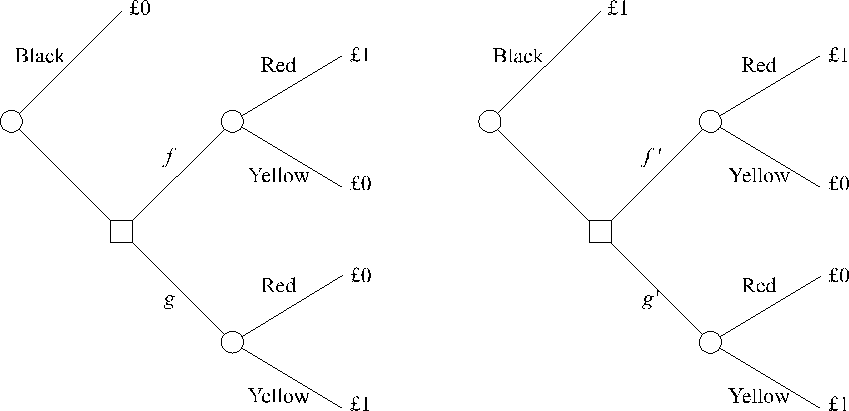
\includegraphics[width=4.16667in,height=\textheight,keepaspectratio]{begging-img1.png}

The left-hand tree represents the choice between \emph{f} and \emph{g}.
The subject is told that if a black ball is drawn they will receive
nothing, but if it is not drawn they will have a choice between betting
on red and betting on yellow. So far we have a standard enough dynamic
choice problem. Maher proposes to make it synchronic by requiring that
subjects specify in advance what they would do if they reached the
square, that is if a black ball is not drawn. This, he claims, makes the
situation exactly as if the agent was choosing between \emph{f} and
\emph{g}. Now the right-hand tree is the same as the left-hand tree in
all respects but one. If a black ball is drawn the agent receives £1,
not nothing. But the only choice the agent has to make is exactly the
same as in the left-hand tree, so they ought make the same choice. We
can concede to Maher here that it would be irrational to specify, in
advance, a preference for \emph{g} over \emph{f} in the left-hand tree
and for \emph{f}′ over \emph{g} in the right-hand tree. This is,
however, insufficient for his conclusion.

The problem lies in his assumption that ``it seems uncontroversial that
the consequences a person values are not changed by representing the
options in a tabular or tree form'' Maher
(\citeproc{ref-Maher1993}{1993, 71}). As Seidenfeld
(\citeproc{ref-Seidenfeld1994}{1994}) makes clear, this is exactly what
is controversial in these circumstances. Indeed this premise, call it
Reduction, is expressly denied by a number of heterodox decision
theorists, and by writers who deny \emph{Addition} on the occasions they
talk about decision theory. There is a good reason for this. As noted
above, on the Dempster-Shafer theory,
\emph{Bel}(\emph{B}\({\vee}\)\emph{R})may be greater than
\emph{Bel}(\emph{B})+\emph{Bel}(\emph{R}). When evaluating the worth of
choosing \emph{f}′ in the original, tabular, it seems plausible that it
is \emph{Bel}(\emph{B}\({\vee}\)\emph{R}) that matters, not
\emph{Bel}(\emph{B})+\emph{Bel}(\emph{R}). However in the tree form
problem all that matters to \emph{f}′ is \emph{Bel}(\emph{B}), for the
possibility that we won't need to choose, and \emph{Bel}(\emph{R}), for
the possibility that we do.

The point is that Maher has to either assume agents only consider
\emph{Bel}(\emph{B}) and \emph{Bel}(\emph{R}) when assessing \emph{f}′,
not \emph{Bel}(\emph{B}\({\vee}\)\emph{R}), or that
\emph{Bel}(\emph{B}\({\vee}\)\emph{R}) is some function of
\emph{Bel}(\emph{B}) and \emph{Bel}(\emph{R}) so that we can ignore that
complication, in his `uncontroversial' assumption. The first option is
implausible, surely when comparing \emph{f}′ and \emph{g}′ we just
compare \emph{Bel}(\emph{B}\({\vee}\)\emph{R}) with
\emph{Bel}(\emph{B}\({\vee}\)\emph{Y}). More interestingly, I claim that
the second is question-begging. Given that virtually everyone agrees
that in some cases, for example lotteries, degrees of belief should be
probability functions, in some cases the function which gives us
\emph{Bel}(\emph{B}\({\vee}\)\emph{R}) from \emph{Bel}(\emph{B}) and
\emph{Bel}(\emph{R}) must be addition. Hence he must assume that
\emph{Bel}(\emph{B}\({\vee}\)\emph{R}) =
\emph{Bel}(\emph{B})+\emph{Bel}(\emph{R}) for the move from tabular to
tree form to be plausible. But this is just what he was trying to prove,
so the argument is question-begging.

\section{Conclusion}\label{conclusion}

Maher rightly objects to depragmatised Dutch Book arguments on the
ground that they are question-begging. That is, they use their
conclusion as an implicit premise. It is argued here that the same
objection applies to Maher's argument for Bayesianism. He relies on the
reducibility of tree form decisions to table form decisions, but the
only justification for this could be a reliance on \emph{Addition}. But
\emph{Addition} was what he was trying to prove all along, so he isn't
allowed to take Reduction as a premise.

There are three moves that Maher could make here. First, he could say
that Reduction is so obvious that it should be acceptable as a premise
without justification. The resulting argument may be effective at
convincing some agnostics about Bayesianism that their implicit
assumptions all along were Bayesian, but it would be completely
ineffective against the sceptics about Bayesianism I have been
discussing. Secondly, he could come up with a new argument for Reduction
that I haven't considered here and isn't vulnerable to this objection.
Given the conclusions of the last section I doubt this is possible, but
the ingenuity of philosophers shouldn't be underestimated. Thirdly, and
most interestingly, he could look for justifications of Bayesianism that
do not rely on construing credences as dispositions to bet. Since the
arguments from considerations about preferences to constraints on
credences have so far all failed, the time might be right to look at the
problem from a different direction.

\subsection*{References}\label{references}
\addcontentsline{toc}{subsection}{References}

\phantomsection\label{refs}
\begin{CSLReferences}{1}{0}
\bibitem[\citeproctext]{ref-Christensen1996}
Christensen, David. 1996. {``Dutch-Book Arguments {D}e-Pragmatized:
Epistemic Consistency for Partial Believers.''} \emph{Journal of
Philosophy} 93 (9): 450--79. doi:
\href{https://doi.org/10.2307/2940893}{10.2307/2940893}.

\bibitem[\citeproctext]{ref-Dempster1967}
Dempster, Arthur. 1967. {``Upper and Lower Probabilities Induced by a
Multi-Valued Mapping.''} \emph{Annals of Mathematical Statistics} 38:
325--39. doi:
\href{https://doi.org/10.1214/aoms/1177698950}{10.1214/aoms/1177698950}.

\bibitem[\citeproctext]{ref-Dempster1968}
---------. 1968. {``A Generalisation of Bayesian Inference.''}
\emph{Journal of the Royal Statistical Society Series B} 30: 205--47.

\bibitem[\citeproctext]{ref-vanFraassen1989}
Fraassen, Bas van. 1989. \emph{Laws and Symmetry}. Oxford: Clarendon
Press.

\bibitem[\citeproctext]{ref-Hart1942}
Hart, A. G. 1942. {``Risk, Uncertainty and the Unprofitability of
Compounding Probabilities.''} In \emph{Studies in Mathematical Economics
and Econometrics}, edited by F. McIntyre O. Lange and T. O. Yntema.,
110--18. Chicago: University of Chicago Press.

\bibitem[\citeproctext]{ref-Hellman1997}
Hellman, Geoffery. 1997. {``Bayes and Beyond.''} \emph{Philosophy of
Science} 64 (2): 191--221. doi:
\href{https://doi.org/10.1086/392548}{10.1086/392548}.

\bibitem[\citeproctext]{ref-HowsonUrbach1989}
Howson, Colin, and Peter Urbach. 1989. \emph{Scientific Reasoning}. La
Salle: Open Court.

\bibitem[\citeproctext]{ref-Jeffrey1983}
Jeffrey, Richard. 1983. {``Bayesianism with a Human Face.''} In
\emph{Testing Scientific Theories}, edited by J. Earman (ed.).
Minneapolis: University of Minnesota Press.

\bibitem[\citeproctext]{ref-Kaplan1993}
Kaplan, Mark. 1993. {``Confessions of a Modest Bayesian.''}
\emph{Canadian Journal of Philosophy} 23 (sup1): 315--37. doi:
\href{https://doi.org/10.1080/00455091.1993.10717353}{10.1080/00455091.1993.10717353}.

\bibitem[\citeproctext]{ref-Kaplan1996}
---------. 1996. \emph{Decision Theory as Philosophy}. Cambridge:
Cambridge University Press.

\bibitem[\citeproctext]{ref-Keynes1937}
Keynes, John Maynard. 1937. {``The General Theory of Employment.''}
\emph{Quarterly Journal of Economics} 51 (2): 209--23. doi:
\href{https://doi.org/10.2307/1882087}{10.2307/1882087}. Reprinted in
\cite[XIV 109-123]{KeynesCW}, references to reprint.

\bibitem[\citeproctext]{ref-Knight1921}
Knight, Frank. 1921. \emph{Risk, Uncertainty and Profit}. Chicago:
University of Chicago Press.

\bibitem[\citeproctext]{ref-Levi1980}
Levi, Isaac. 1980. \emph{The Enterprise of Knowledge}. Cambridge, MA.:
MIT Press.

\bibitem[\citeproctext]{ref-Maher1993}
Maher, Patrick. 1993. \emph{Betting on Theories}. Cambridge: Cambridge
University Press.

\bibitem[\citeproctext]{ref-Maher1997}
---------. 1997. {``Depragmatised Dutch Book Arguments.''}
\emph{Philosophy of Science} 64 (2): 291--305. doi:
\href{https://doi.org/10.1086/392552}{10.1086/392552}.

\bibitem[\citeproctext]{ref-Savage1954}
Savage, Leonard. 1954. \emph{The Foundations of Statistics}. New York:
John Wiley.

\bibitem[\citeproctext]{ref-Schick1986}
Schick, Frederick. 1986. {``Dutch Bookies and Money Pumps.''}
\emph{Journal of Philosophy} 83 (2): 112--19. doi:
\href{https://doi.org/10.2307/2026054}{10.2307/2026054}.

\bibitem[\citeproctext]{ref-Seidenfeld1994}
Seidenfeld, Teddy. 1994. {``When Normal and Extensive Form Decisions
Differ.''} In \emph{Logic, Methodology and Philosophy of Science},
edited by Brian Skyrms Dag Prawitz and Dag Westerståhl, 451--63.
Amsterdam: Elsevier.

\bibitem[\citeproctext]{ref-Shafer1976}
Shafer, Glenn. 1976. \emph{A Mathematical Theory of Evidence}.
Princeton: Princeton University Press.

\bibitem[\citeproctext]{ref-Tintner1941}
Tintner, Gerhard. 1941. {``The Theory of Choice Under Subjective Risk
and Uncertainty.''} \emph{Econometrica} 9 (3/4): 298--304. doi:
\href{https://doi.org/10.2307/1907198}{10.2307/1907198}.

\bibitem[\citeproctext]{ref-Walley1996}
Walley, Peter. 1996. {``Inferences from Multinomal Data: Learning about
a Bag of Marbles (with Discussion).''} \emph{Journal of the Royal
Statistical Society Series B} 58: 3--57.

\bibitem[\citeproctext]{ref-Yager1994}
Yager, R., M. Fedrizzi, and J. Kacprzyk, eds. 1994. \emph{Advances in
the Dempster- Shafer Theory of Evidence}. New York: John Wiley.

\end{CSLReferences}



\noindent Published in\emph{
Studies in History and Philosophy of Science Part A}, 2001, pp. 687-697.


\end{document}
